%%%%%%%%%%%%%%%%%%%%%%%%%%%%%%%%%%%%%%%%%%%%%%%%%%%%%%%%%%%%%%%%%%%%%%%%%%
 %																		%
 %	Plantilla Latex para presentación del proyecto de curso				%
 %	Programación de Aplicaciones para Internet y la Nube					%
 %																		%
 %	Creada por: Duván Pardo, Wilson López								%
 %																		%
 %	Versión: 0.2															%
 %	Dapardoc@gmail.com ; Wilrilo@gmail.com								%
 %																		% 
 %	Se requieren los archivos  plantilla.bbl								% 
 %	El directorio Imagenes que contiene: CECAD,DC, Elementos y RITA		%  
 %																		%
%%%%%%%%%%%%%%%%%%%%%%%%%%%%%%%%%%%%%%%%%%%%%%%%%%%%%%%%%%%%%%%%%%%%%%%%%%

\documentclass[10pt]{article}   			% Describe el tipo de documento, y el tamaño de la letra del texto

\usepackage[utf8]{inputenc}				% Define codificación para que permita caracteres latinos (acentos)
\usepackage[spanish,activeacute]{babel} 	% Paquete para poder escribir con tildes y otros caracteres especiales

\usepackage{vmargin}						% Código para margenes y formato de página
\setpapersize{A4}
\setmargins	{2.2cm}     					% margen izquierdo
			{1 cm}                 		% margen superior
			{16.5cm}               		% anchura del texto
			{23.42cm}             		% altura del texto
			{20pt}                		% altura de los encabezados
			{1.2cm}               		% espacio entre el texto y los encabezados
			{0pt}                		% altura del pie de página
			{2cm}                 		% espacio entre el texto y el pie de página

\usepackage{amsmath}						% paquete para expresiones matemáticas
\usepackage{amsfonts}					% paquete para escritura de ecuaciones 
\usepackage{amssymb}						% paquete para caracteres especiales para ecuaciones 

\usepackage{fancyhdr}					% Temas para encabezado y pie de pagina
\usepackage{fancyvrb}
\pagestyle{fancy} 

\pagenumbering{arabic} 					% Numeración de paginas {arabic roman}
\usepackage{hyperref}					% Para hipervinculos
\usepackage{graphicx}					% Para incluir imágenes
\usepackage{caption}						% Descripciones de las figuras
\usepackage{subcaption}					% Descripción varias imagenes en usa sola figura
\graphicspath{ {Imagenes/} }				% Directorio de imágenes esta capeta va donde esta el archivo tex


\usepackage{color, colortbl}				% Colores para tablas
\usepackage{listings}					% Para el código Fuente
\usepackage{xcolor}						% para color en codigos o listrings
\definecolor{limegreen}{RGB}{50,100,50}	% Definición de colores ejemplo verde en RGB
\definecolor{Red}{RGB}{220,120,120}		% se definen colores para la tabla en el cronograma pueden ser RGB 0-255 o rgb 0-1 cada componente
\definecolor{LightCyan}{rgb}{0.88,1,1}
\definecolor{azul}{RGB}{120,120,210}
\lstdefinestyle{base}{
	language=C,
	emptylines=1,
	breaklines=true,
	showspaces=fasle,
	showstringspaces=false,
	extendedchars=true,
	basicstyle=\ttfamily\color{black},
	moredelim=**[is][\color{limegreen}]{'}{'}, 	% Para este caso especial el caracter ' y & encierran
	moredelim=**[is][\color{blue}]{&}{&},		% un fragmento de código que quiere ser coloreado
}

\lstset{numbers=left, numberstyle=\tiny, stepnumber=2, numbersep=5pt}

%Aquí inicia el documento.
\begin{document}
	% Se define el Encabezado
	%clhead[]{Proyecto}
	\lhead[]{Programación de Aplicaciones para Internet y la Nube}
	\rhead[]{\textbf{2016-I}}
	\renewcommand{\headrulewidth}{0.5pt}

	\thispagestyle{empty}						% La primera página no lleva estilo (sin encabezado)
	\begin{center}
		\large {Programación de Aplicaciones para Internet y la Nube
			\hspace{5 cm}\textbf{2016-I}}
		\bigskip  
		\textbf{
			\LARGE{\\NOMBRE DEL PROYECTO}}\\								% Nombre del proyecto
	\end{center}	
	\begin{flushright}	
		\bigskip	
		Nombre del Estudiante: \textbf{Duván Pardo, Wilson López}			% Nombre del estudiante
	\end{flushright} 
	
\section{Introducción}

De manera general  hable sobre el  contexto del tema que se va a trabajar. es prudente agregar algunas referencias.
		
\section{Descripción del proyecto}

En esta sección se realiza una descripción del proyecto, El proyecto de curso, deberá ser realizado de manera individual. A continuación, se proveen algunas sugerencias de carácter general para su realización. Los temas, y en el ámbito conceptual de los mismos, los tipo de proyectos sugeridos son los siguientes, siguiendo el marco de la Programación de Aplicaciones para Internet y la Nube:
		
\begin{itemize}
	\item Internet de las Cosas (IoT) y Computación en Nube para el Hogar Inteligente (Smart Home)
	\item Internet de las Cosas (IoT) y Computación en Nube para el Edificio Inteligente (SmartBuilding)
	\item Internet de las Cosas (IoT) y Computación en Nube para control del ciclo de desarrollo de la construcción mediante el Modelo de Información de Edificación			
	\item Internet de las Cosas (IoT) y Computación en Nube para Servicios Basados en la Localización (LBSs)
	\item Internet de las Cosas (IoT) y Computación en Nube con base en Wireless Sensor Networks (WSNs)
	\item Internet de las Cosas (IoT) y Computación en Nube hacia infraestructuras para e-Ciencia.
	\item Internet de las Cosas (IoT) y Computación en Nube hacia Massive Online Courses(MOOCs).
	\item Internet de las Cosas (IoT) y Computación en Nube hacia Big Data Analytics
	\item Internet de las Cosas (IoT) y Computación en Nube hacia Movilidad Inteligente
	\item Internet de las Cosas (IoT) y Computación en Nube hacia el procesamiento masivo de datos procedentes de drones			
	\item Internet de las Cosas (IoT) y Computación en Nube para Infrmática Forense en la época del postconflicto colombiano			
\end{itemize}
		
\begin{figure}[ht] % Es preferible verificar la documentación para que la imagen quede correctamente segun el parámetro entre []
	\centering
		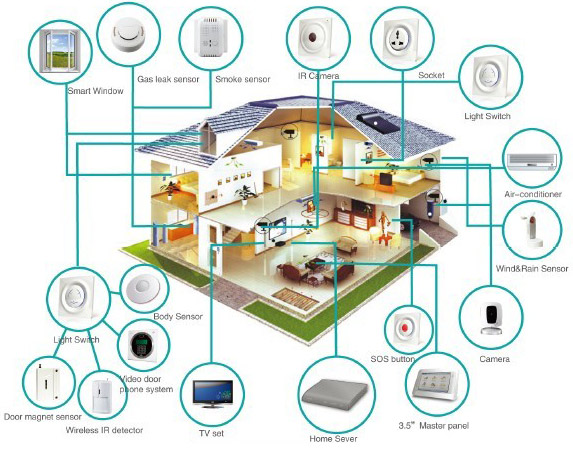
\includegraphics[scale=0.25]{Elementos}   % Scale se utiliza para cambiar el tamaño de la imagen
	\caption{en esta parte va la descripción de la imagen, colocar fuente: si es adaptada que diga adaptación del autor, se recomienda que la imagen sea vectorizadas formato .eps} \label{fig:Elementos}
\end{figure}
		
\newpage % Se utiliza para escribir en una nueva pagina (estilo)

\section{Objetivos}

\subsection{General}

	\begin{itemize}
		\item Debe indicar explícitamente lo que se quiere lograr con el proyecto. Coincide con el título del proyecto.
	\end{itemize}
	
\subsection{Especificos}

	\begin{itemize}
		\item Son la descomposición y secuencia lógica del objetivo general, son aquellos por los cuales se puede lograr el objetivo general.
		\item Es recomendable no tener muchos objetivos específicos (máximo 4).
		\item Se deben redactar en forma afirmativa, en tiempo verbal infinitivo, sujetos a una sola interpretación.
	\end{itemize}
		
\section{Recursos}

En esta sección se mencionan los recursos requeridos entre los que cuenta la Universidad Distrital están el Centro de Cómputo de Alto Desempeño CECAD y la Red de investigaciones de Tecnología avanzada RITA, para la implementación de sistemas en nube y si es posible el acceso a pruebas sobre IPv6.
		
% se muestra un ejemplo de una imagen con sub figuras, caption y subcaption para sus respectivas descripciones
\begin{figure}[ht]
\centering
\begin{subfigure}[b]{0.4\textwidth}  		% el nunero se utiliza para cambiar la escala de la imagne
	
\includegraphics[width=\textwidth]{RITA}
	\caption{RITA}
	\label{fig:RITA}
\end{subfigure}
\begin{subfigure}[b]{0.4\textwidth}		 	% el nunero se utiliza para cambiar la escala de la imagne
	
\includegraphics[width=\textwidth]{CECAD}
	\caption{CECAD}
	\label{fig:CECAD}
\end{subfigure}
\begin{subfigure}[b]{0.9\textwidth}		 	% el nunero se utiliza para cambiar la escala de la imagne
	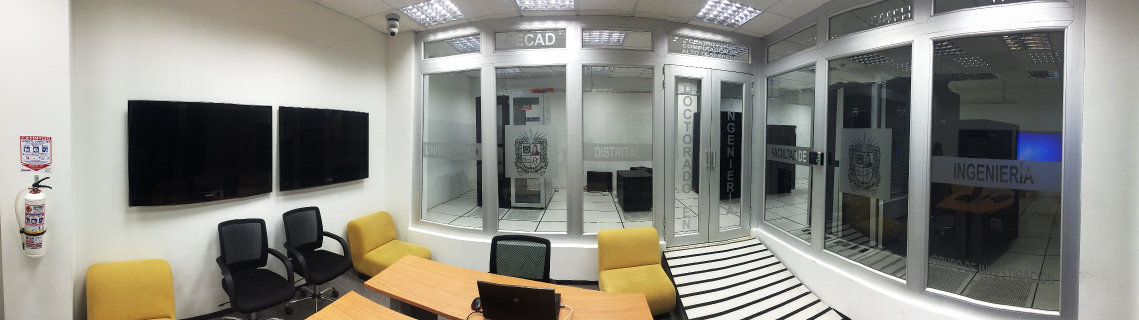
\includegraphics[width=\textwidth]{DC}
	\caption{Data Center Doctorado en Ingeniería Universidad Distrital - CECAD}
	\label{fig:DC}
\end{subfigure}
\caption{Recursos dentro de la Universidad Distrital.}\label{fig:Recursos Universidad Distrital.}
\end{figure}

\newpage % Se utiliza para escribir en una nueva pagina (estilo)

\section{Cronograma}	
	
\newcolumntype{g}{>{\columncolor{Red}}l} % si se quiere dar color se crea un estilo en este caso "g"
\begin{table}[ht]
	\centering 
	\begin{small}
	\setlength{\tabcolsep}{3pt}
	\begin{tabular}{|l|c|c|c|c|g|c|c|c|c|c|c|c|c|c|c|c|c|c|c|c|c|c|c|}\hline % cuando se define estilo se cambia por una g
	\rowcolor{LightCyan}
	&\multicolumn{10}{c|}{\textbf{Semana}}\\ \cline{2-11}
	\rowcolor{LightCyan} 										% para aplicar color en una fila
	\raisebox{1.5ex}{\textbf{Actividades}}					
																	&  01 & 02 & 03 & 04 & 05 & 06 & 07 & 08 & 09 & 10 \\ \hline
Plantear y programar estructura de orquestación
																	& X & X & X & X & X & X & X & & &  \\ \hline
\cellcolor{azul} 															% si se quiere color en unsa sola celda	
Programar servidor de almacenamiento
																	& & & X & X & X & X & & & &  \\ \hline
Programar servidor de recepción de información
																	& & & X & X & X & X & X & X & &  \\ \hline
Programar servidor de envío de correos
																	& & & & & X & X & X & X & & \\ \hline
programar sistemas embebidos
																	& & & X & X & X & X & X & X & X & \\ \hline
realización de pruebas y corrección de errores
																	& & & & X & X & X & X & X & X & X \\ \hline
	\end{tabular} 
	\end{small}
	\caption{Cronograma de actividades}
	\label{t_cronograma}
\end{table} 
	
\section{Resultados Esperados}

Resultado esperado la idea es que se den cuenta que programamos para Internet y la nube que se entiende Internet por internet de la nube, si es visualización de  plataformas o software para servicios, se tiene que trabajar en cecad pero también es importante llevarlo a la nube pública Amazon, Azure entre otras.
		
\section{Programación Literaria dentro del informe final}

Ejemplo para mostrar código en \LaTeX(el sistema reconoce y muestra las tabulaciones).
\begin{small}
\begin{lstlisting}[frame=single,style=base]	
  %%
	# &code here&


// Ejemplo en C
'int' &i&=1;
'for'(&i&=0;&i&<10;&i++&){
	'print'('i');
}
\end{lstlisting}
\end{small}
		
\section{Bibliografía}	
\textbf{{\Large Accesos WEB}}
\begin{itemize}
	\item \href{http://texblog.org/2012/12/21/multi-column-and-multi-row-cells-in-latex-tables/}{Tablas de \LaTeX}
	\item \href{https://en.wikibooks.org/wiki/LaTeX/Hyperlinks}{HiperVinculos en \LaTeX}
	\item \href{https://es.sharelatex.com/learn/Inserting_Images}{Imágenes en \LaTeX}
	\item \href{http://logistica.fime.uanl.mx/miguel/docs/BibTeX.pdf}{Bibliografía en \LaTeX 1}
	\item \href{http://minisconlatex.blogspot.com.co/2011/03/bibliografia.html}{Bibliografía en \LaTeX 2}
\end{itemize}

\bibliographystyle{apalike}						% Estilo de la bibliografía o referencias
\bibliography{biblio}							% Se muestra desde el fichero .bbl
\nocite{*}

\end{document}
